\section{Material Suplementar}

\begin{slide}{Resultados — Busca de Hiperparâmetros (Tabela Completa)}
  \centering
  \scriptsize
  \renewcommand{\arraystretch}{0.85}
  \resizebox{0.98\textwidth}{!}{%
  \begin{tabular}{p{2.8cm} p{9.5cm}}
    \rowcolor{poliBlue!20}
    \textbf{Família/modelo} & \textbf{Espaço de busca avaliado} \\
    \hline
    OLS & Sem hiperparâmetros (referência linear). \\
    \rowcolor{gray!5}
    Ridge & $\alpha \in \{10^{-3},10^{-2},10^{-1},1,10,100\}$. \\
    Lasso & $\alpha \in \{10^{-4},10^{-3},10^{-2},10^{-1},1\}$. \\
    \rowcolor{gray!5}
    ElasticNet & $\alpha \in \{10^{-4},\ldots,1\}$; $l_1\text{-ratio} \in \{0{,}1,\ldots,0{,}9\}$. \\
    \midrule
    \rowcolor{orange!6}
    DT / RF / GB & Profundidade, folhas, nº estimadores, learning rate (grades discretas). \\
    \midrule
    \rowcolor{blue!6}
    KerasMLP & Arquiteturas $(32,)$ a $(512,256,128)$; ativação, LR, L2, batch; Random Search. \\
    \midrule
    \rowcolor{green!6}
    Híbridos (Phy*) & Busca restrita em L2 (e $\omega$ no PhyLoss); arquitetura baseline fixa. \\
    \bottomrule
  \end{tabular}%
  }
  \vfill
  {\scriptsize Fonte: elaborado pela autora.}
\end{slide}
%========================================================================

\begin{slide}{Resultados — Seleção de Preditores (Best Subset)}
  \centering
  \scriptsize
  Busca exaustiva das $2^5$ combinações de variáveis de entrada com regressão linear e GroupKFold.
  \vfill
  \centering
  \begin{tabular}{c c c c c c c}
    \toprule
    $k$ & Subconjunto & RMSE$_{Flux}$ & RMSE$_{Alim}$ & RMSE$_{Ref}$ & R$^2_{Flux}$ & R$^2_{Alim}$ \\
    \midrule
    3 & Ref\_T\_in, Alim\_T\_in, C\_NaCl & 0,222 & 0,625 & 0,604 & 0,744 & 0,817 \\
    4 & + Ref\_V\_in & 0,142 & 0,389 & 0,398 & 0,887 & 0,909 \\
    5 & + P\_vacuum (todos) & \textbf{0,082} & \textbf{0,227} & \textbf{0,242} & \textbf{0,953} & \textbf{0,960} \\
    \bottomrule
  \end{tabular}
  \vfill
  {\footnotesize Conclusão: as 5 variáveis físicas originais já eram o conjunto ótimo. Fonte: Apêndice A do TCC.}
\end{slide}
%========================================================================

\begin{slide}{Resultados — Discretização (Binning)}
  \centering
  \scriptsize
  Avaliação de 32 configurações de discretização (Gaussian Mixture) para cada variável de entrada.
  \vfill
  \centering
  \begin{tabular}{lcccc}
    \toprule
    \textbf{Alvo} & \textbf{Rank} & \textbf{Configuração} & \textbf{RMSE} & \textbf{R$^2$} \\
    \midrule
    Flux & 1 & Baseline (contínuo) & 0,0821 & 0,914 \\
    Flux & 2 & Ref\_T\_in discretizada & 0,0822 & 0,914 \\
    \midrule
    Alim\_T\_out & 1 & Alim\_T\_in discretizada & 0,452 & 0,966 \\
    Alim\_T\_out & 2 & Baseline (contínuo) & 0,514 & 0,955 \\
    \midrule
    Ref\_T\_out & 1 & Ref\_V\_in, C\_NaCl discretizados & 0,142 & 0,996 \\
    Ref\_T\_out & 3 & Baseline (contínuo) & 0,148 & 0,996 \\
    \bottomrule
  \end{tabular}
  \vfill
  {\footnotesize Nenhuma configuração discretizada melhorou consistentemente os 3 alvos simultaneamente. Dados mantidos contínuos. Fonte: Apêndice A do TCC.}
\end{slide}
%========================================================================

\begin{slide}{Resultados — Data Augmentation}
  \centering
  \scriptsize
  Comparação entre modelos treinados apenas com dados experimentais reais e com dados reais + sintéticos.
  \vfill
  \centering
  \begin{tabular}{llccc}
    \toprule
    \textbf{Alvo} & \textbf{Modelo} & \textbf{Treino} & \textbf{RMSE} & \textbf{R$^2$} \\
    \midrule
    Flux & Reg. Linear & Real & 0,077 & 0,965 \\
    Flux & Reg. Linear & Real + Sintético & 0,077 & 0,965 \\
    Flux & MLP & Real & 0,053 & 0,983 \\
    Flux & MLP & Real + Sintético & 0,077 & 0,965 \\
    \midrule
    Alim\_T\_out & Reg. Linear & Real & 0,165 & 0,973 \\
    Alim\_T\_out & MLP & Real & 0,106 & 0,989 \\
    Alim\_T\_out & MLP & Real + Sintético & 0,287 & 0,918 \\
    \midrule
    Ref\_T\_out & Reg. Linear & Real & 0,170 & 0,998 \\
    Ref\_T\_out & MLP & Real + Sintético & 0,262 & 0,995 \\
    \bottomrule
  \end{tabular}
  \vfill
  {\footnotesize Dados sintéticos não trouxeram melhoria consistente; em alguns casos degradaram o desempenho. Fonte: Apêndice A do TCC.}
\end{slide}
%========================================================================

\begin{slide}{Apêndice — RMSE por Target (Agrupado)}
  \centering
  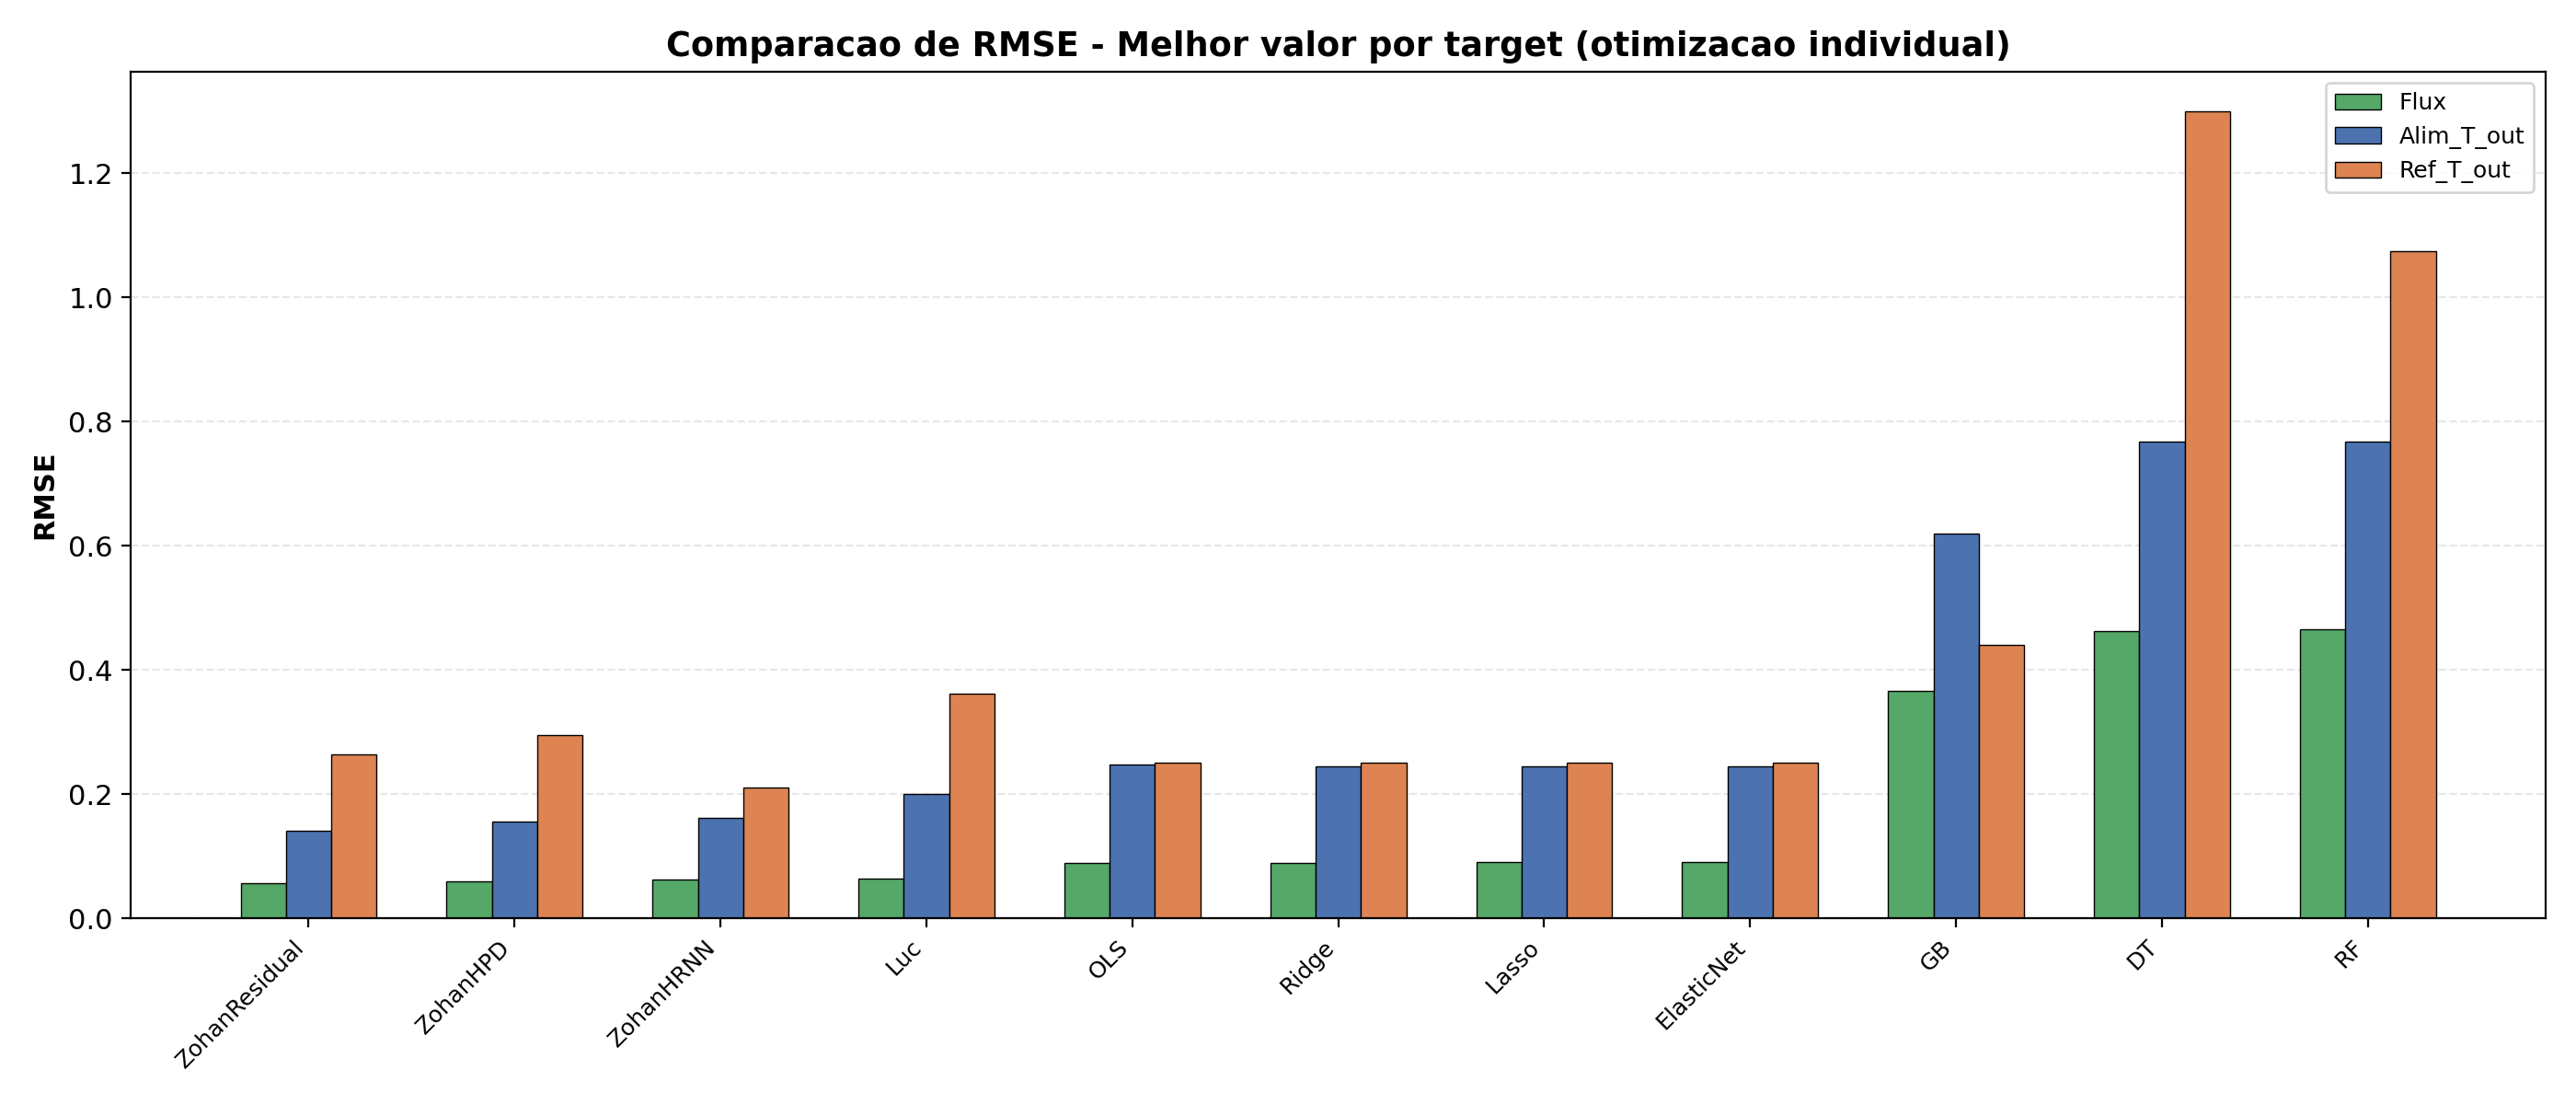
\includegraphics[width=0.75\textwidth]{tcc_images/chap06/model_selection/rmse_by_target_grouped_n.png}
\end{slide}
%========================================================================
\begin{slide}{Apêndice — Melhor RMSE por Família}
  \centering
  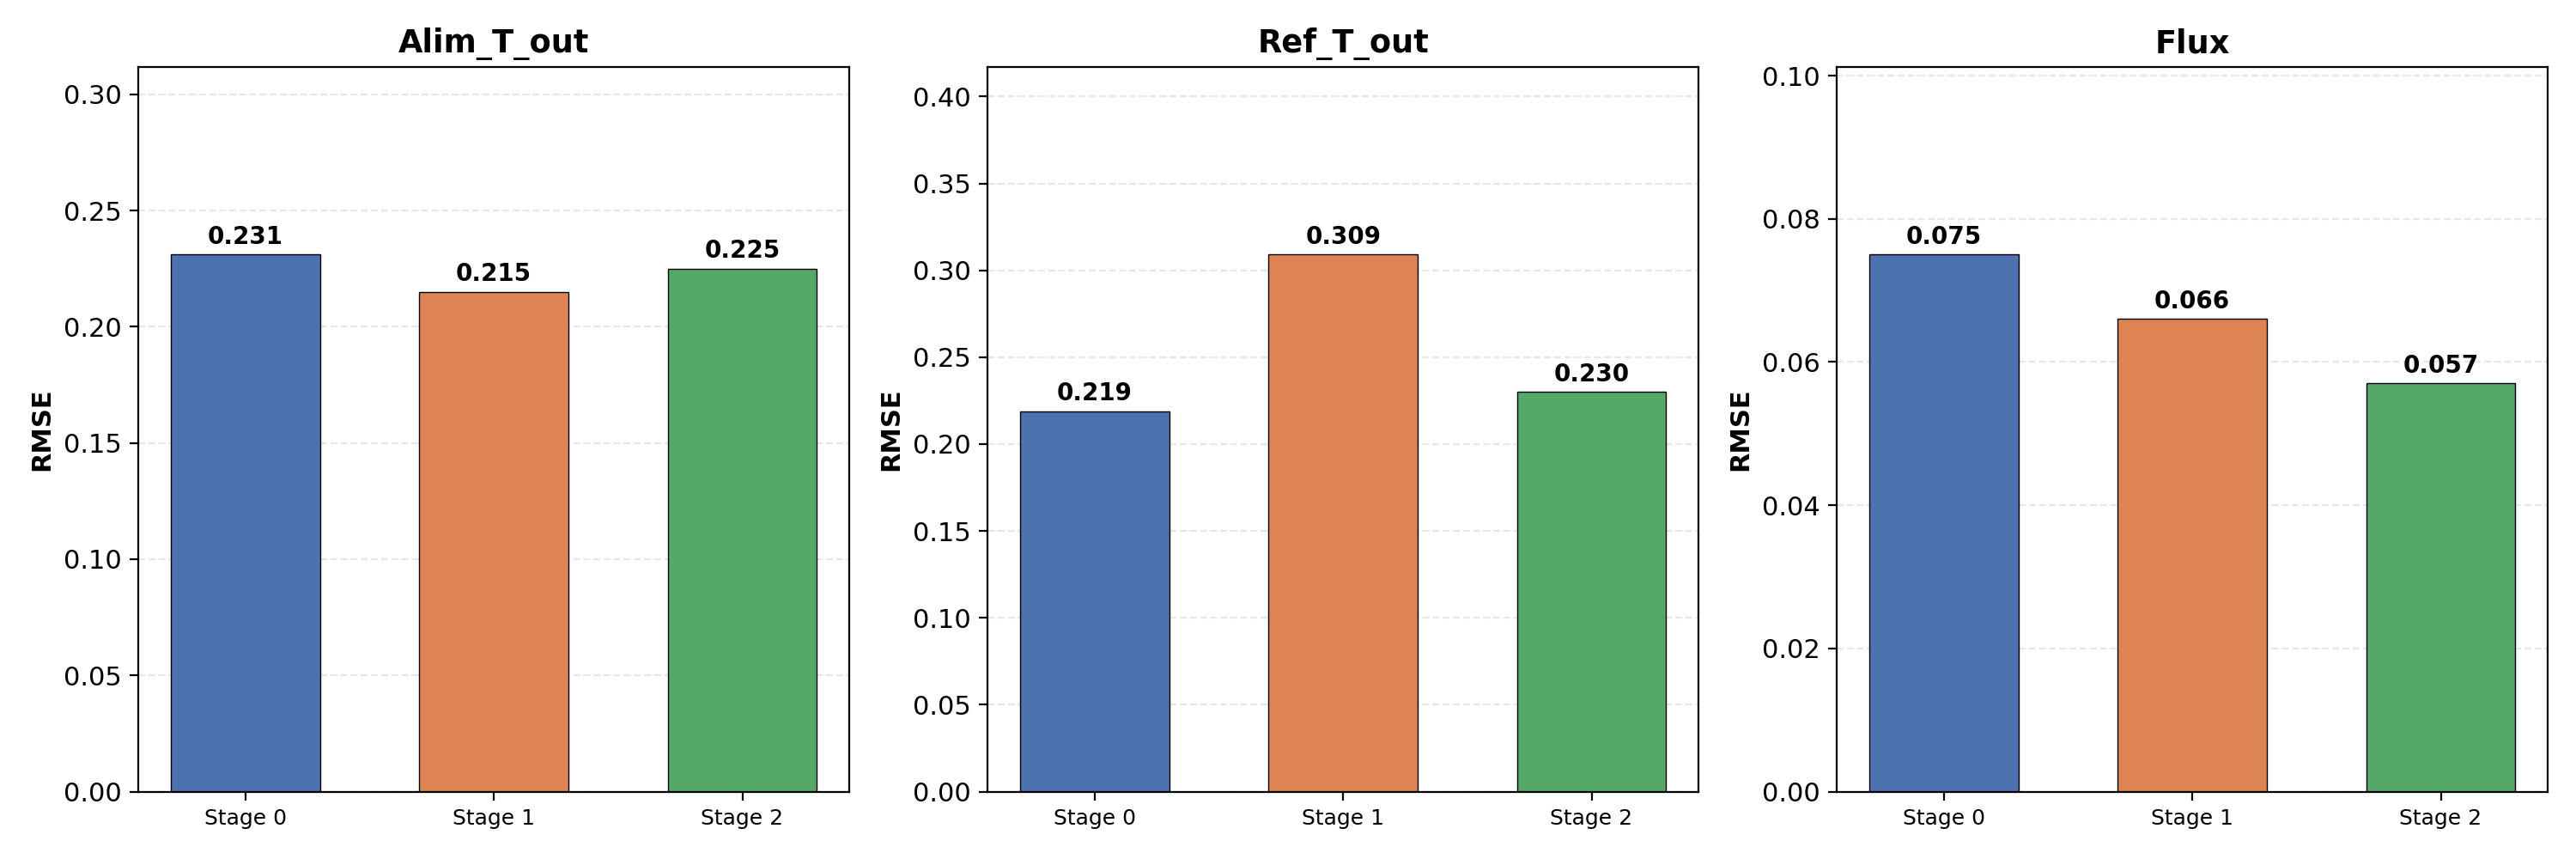
\includegraphics[width=0.85\textwidth]{tcc_images/chap06/best_per_family_rmse_n_v2.png}
\end{slide}
%========================================================================
\begin{slide}{Apêndice — Ranking RMSE (Flux)}
  \centering
  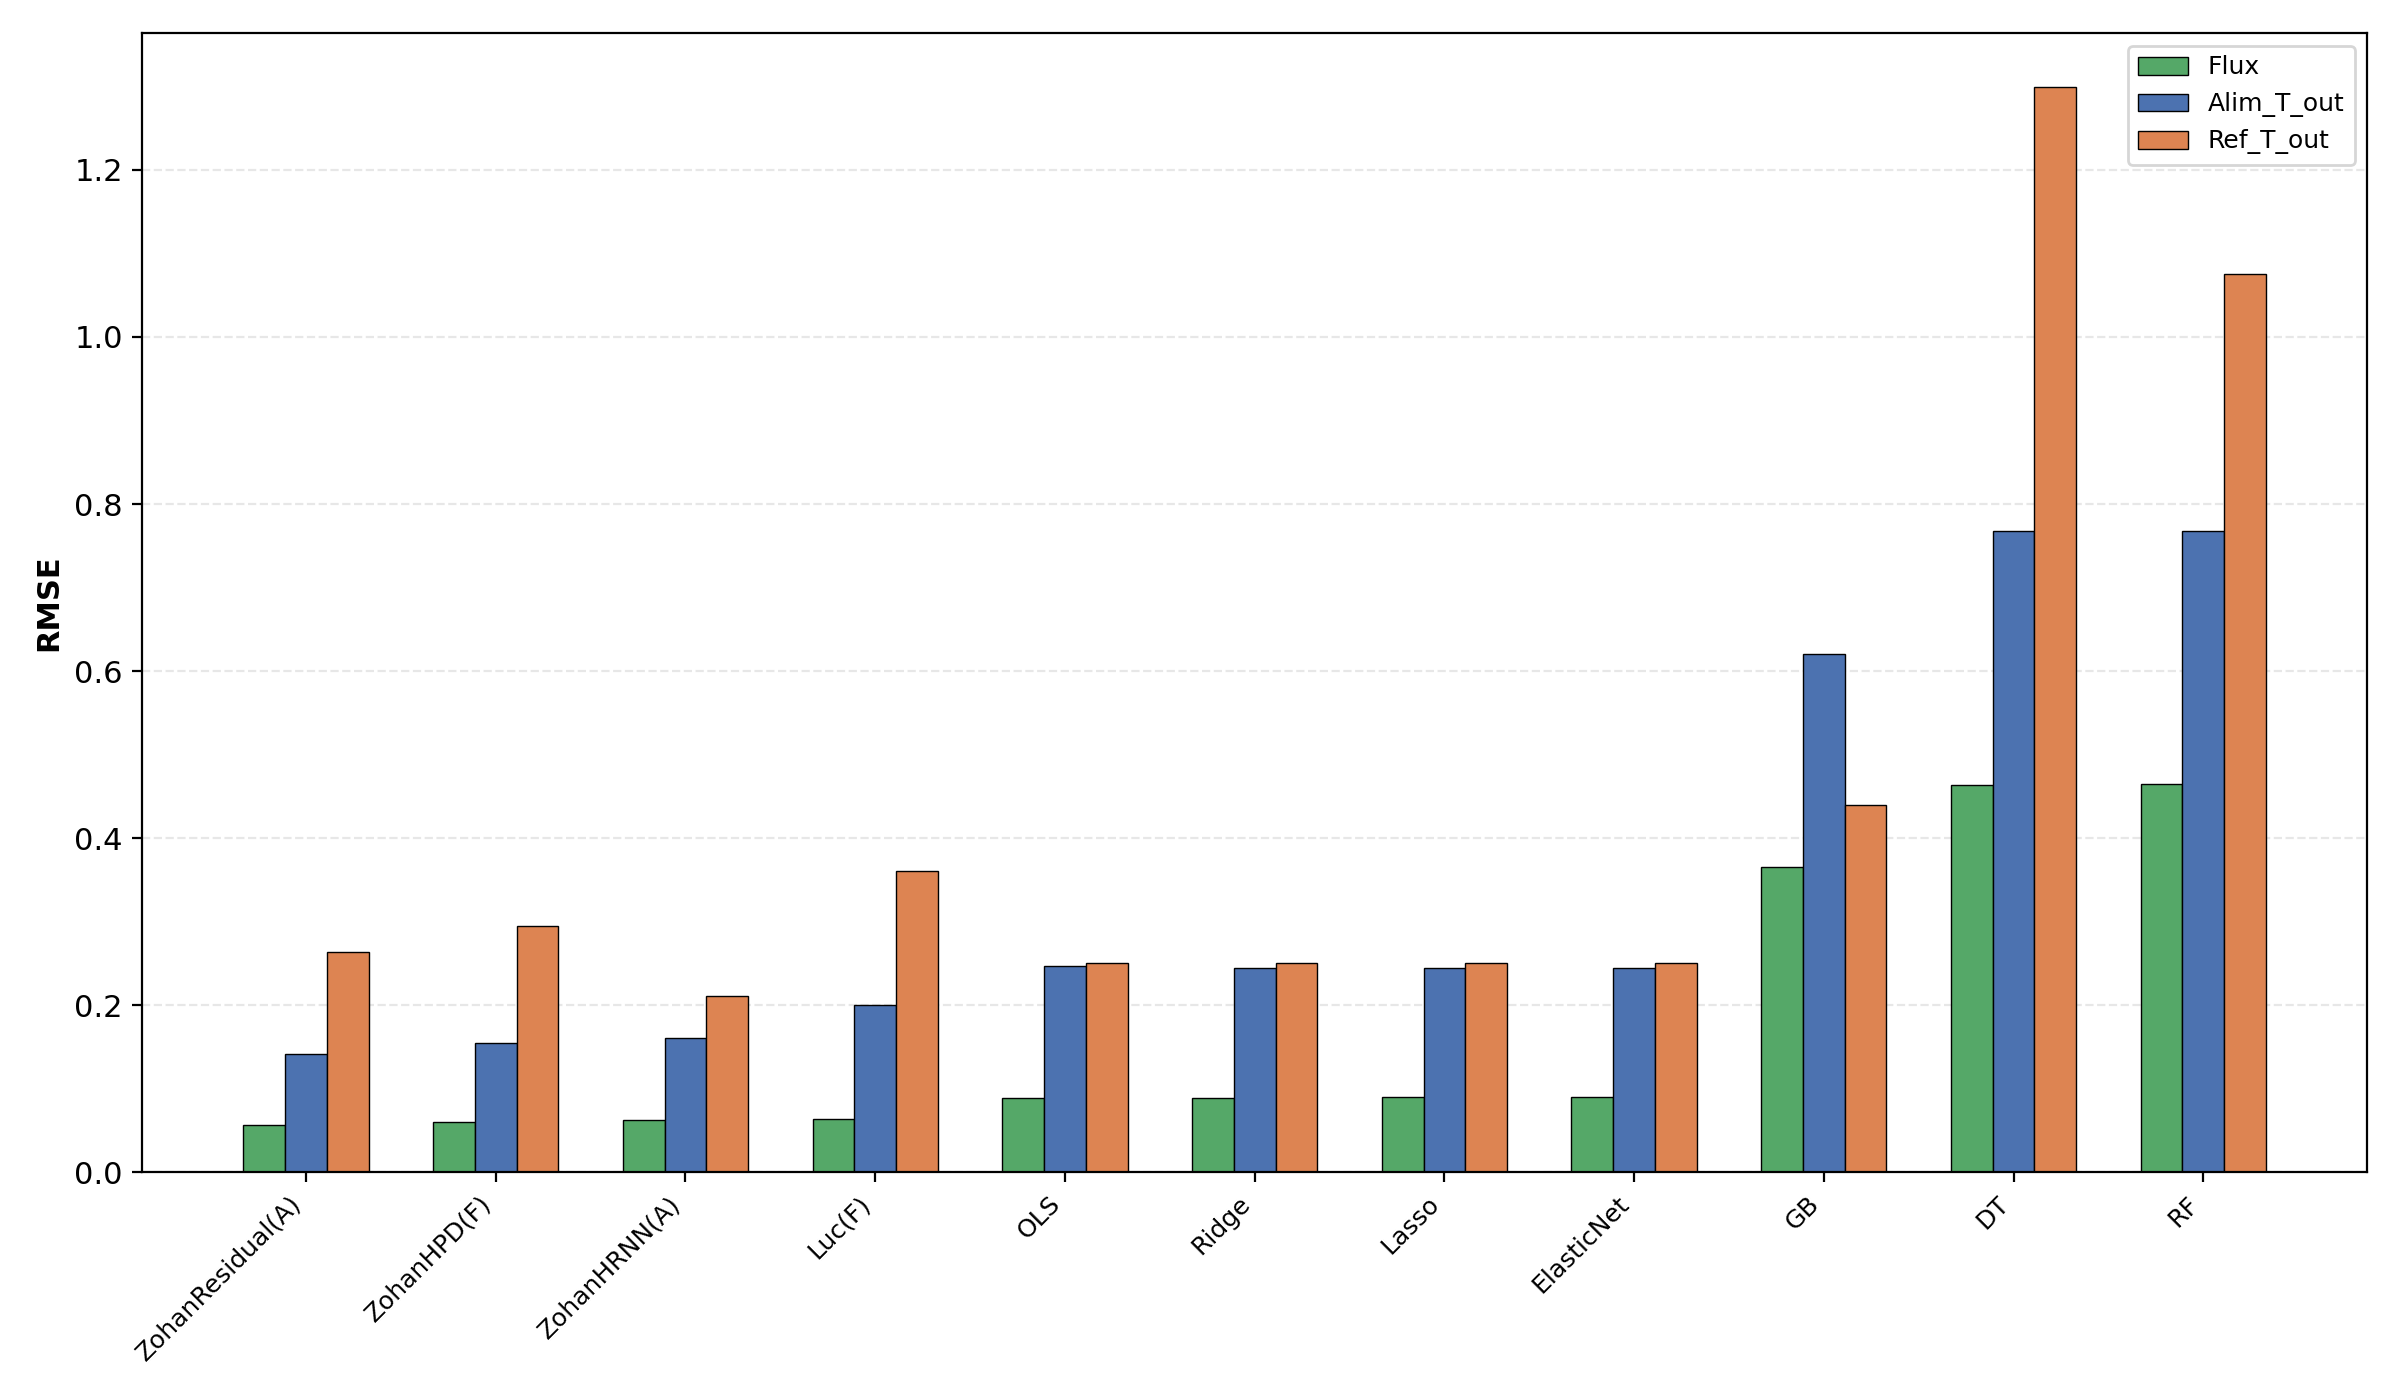
\includegraphics[width=0.85\textwidth]{tcc_images/chap06/ranking_rmse_flux_n.png}
\end{slide}
%========================================================================
\begin{slide}{Apêndice — Varredura de Hiperparâmetros (Learning Rate)}
  \centering
  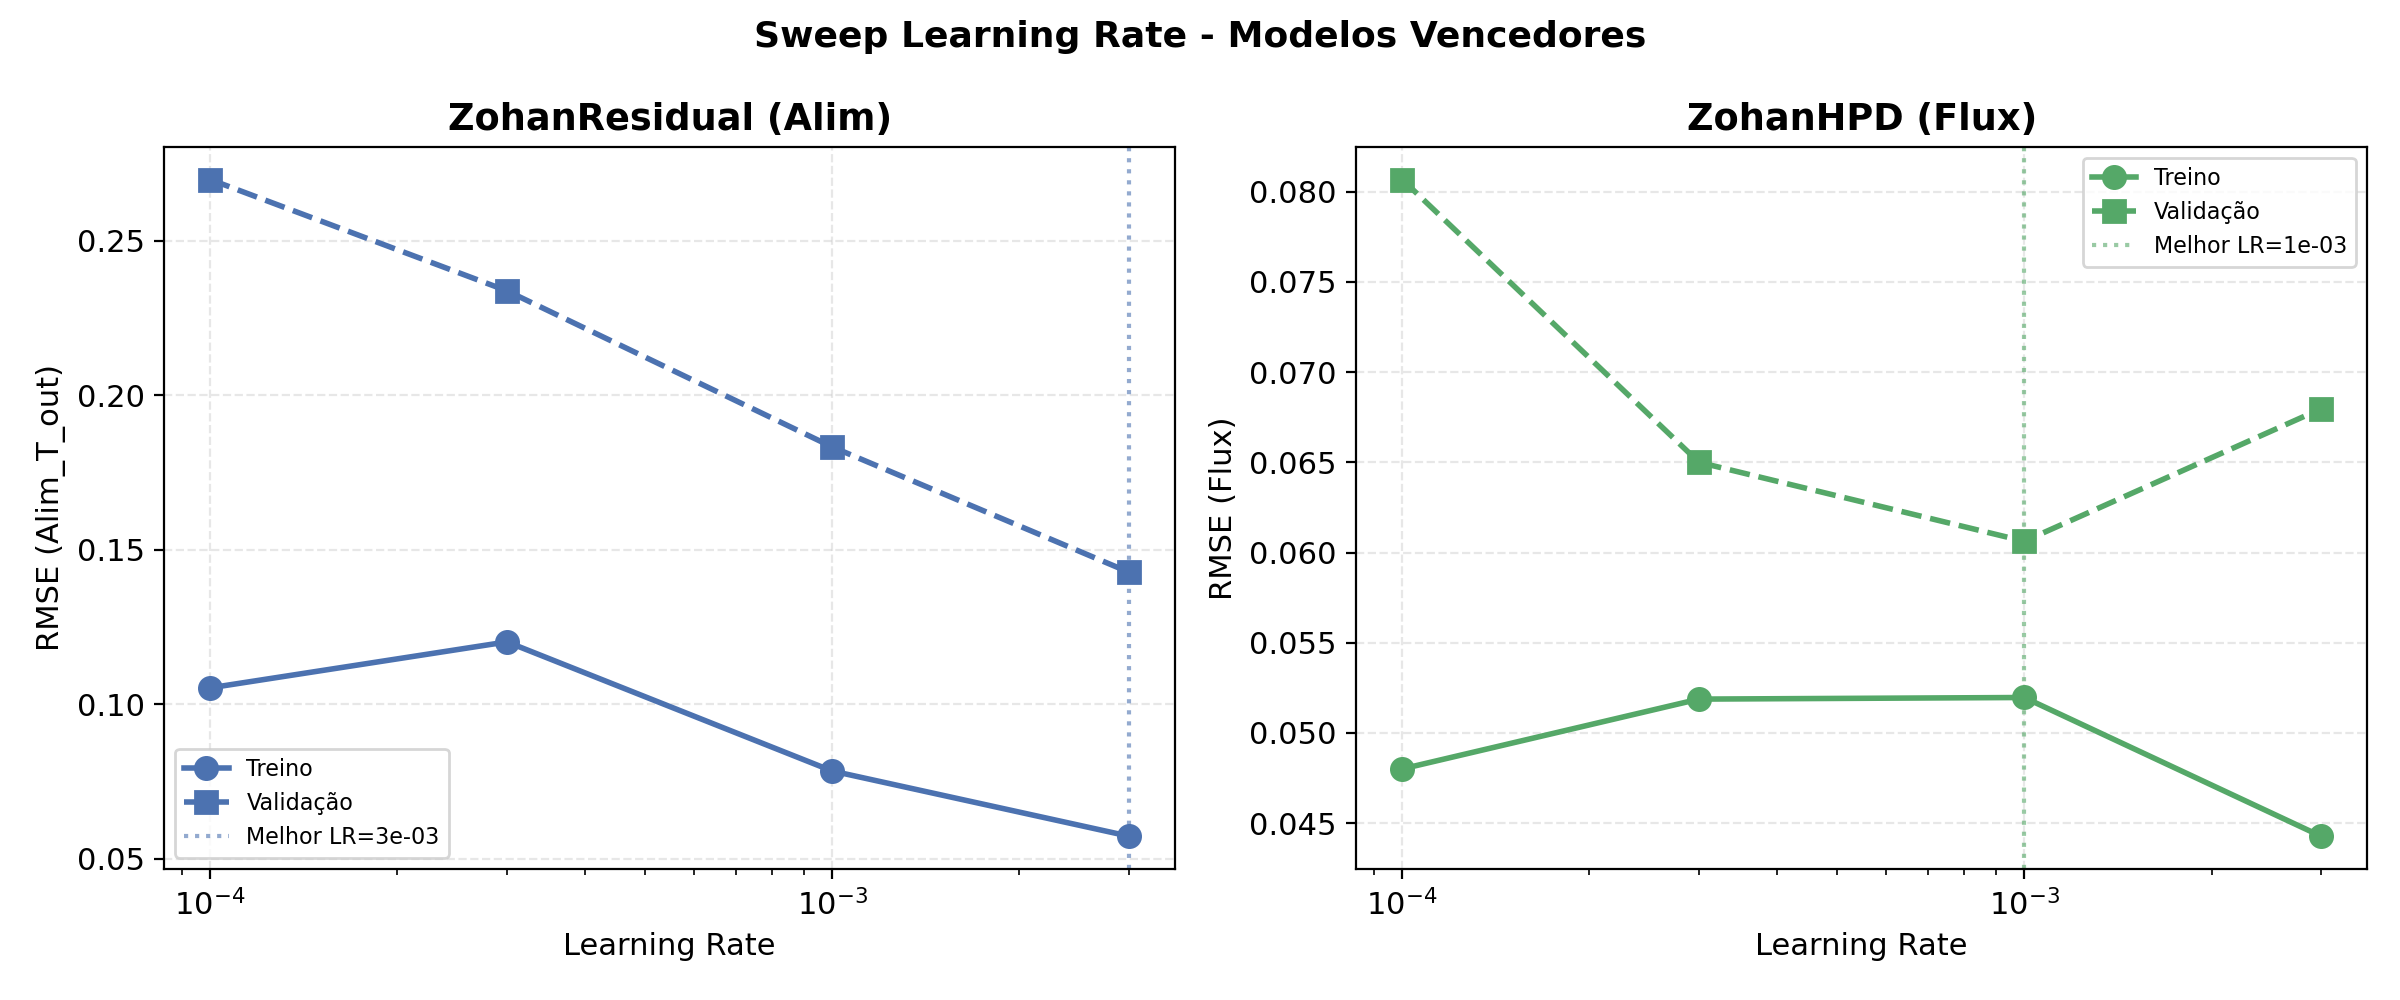
\includegraphics[width=0.85\textwidth]{tcc_images/chap06/model_selection/sweep_lr_winners_n.png}
\end{slide}
%========================================================================
\begin{slide}{Apêndice — Varredura de Hiperparâmetros (L2)}
  \centering
  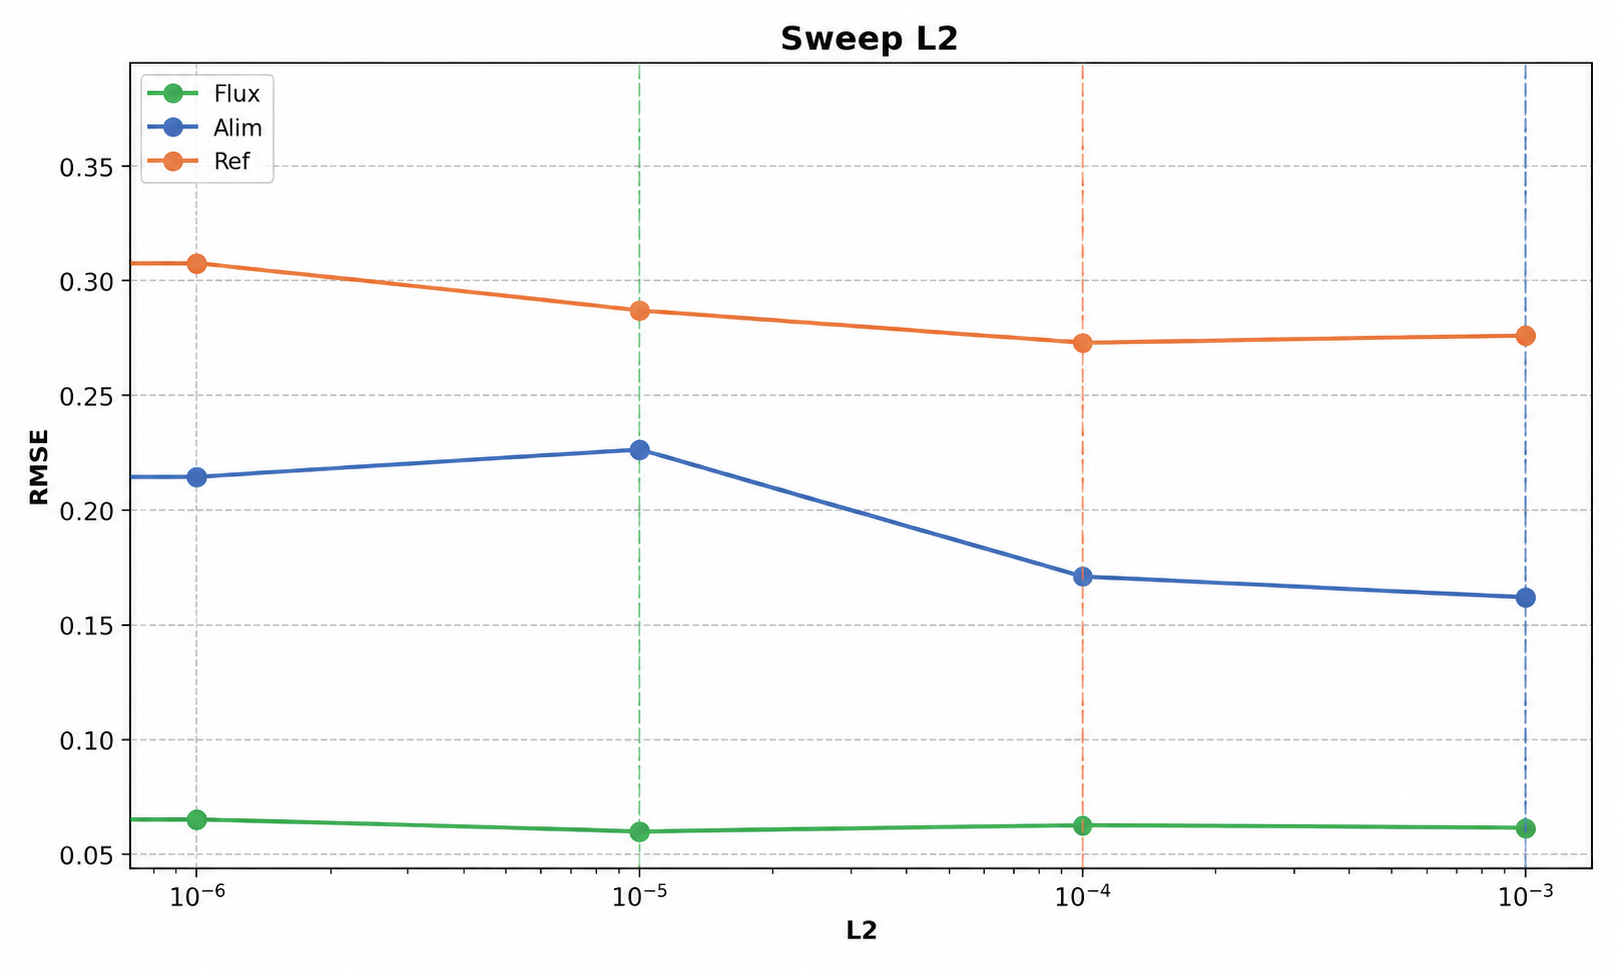
\includegraphics[width=0.85\textwidth]{tcc_images/chap06/model_selection/sweep_l2_winners_n_v2.png}
\end{slide}
%========================================================================
\begin{slide}{Apêndice — Seleção de Hiperparâmetros (PhyResidual)}
  \centering
  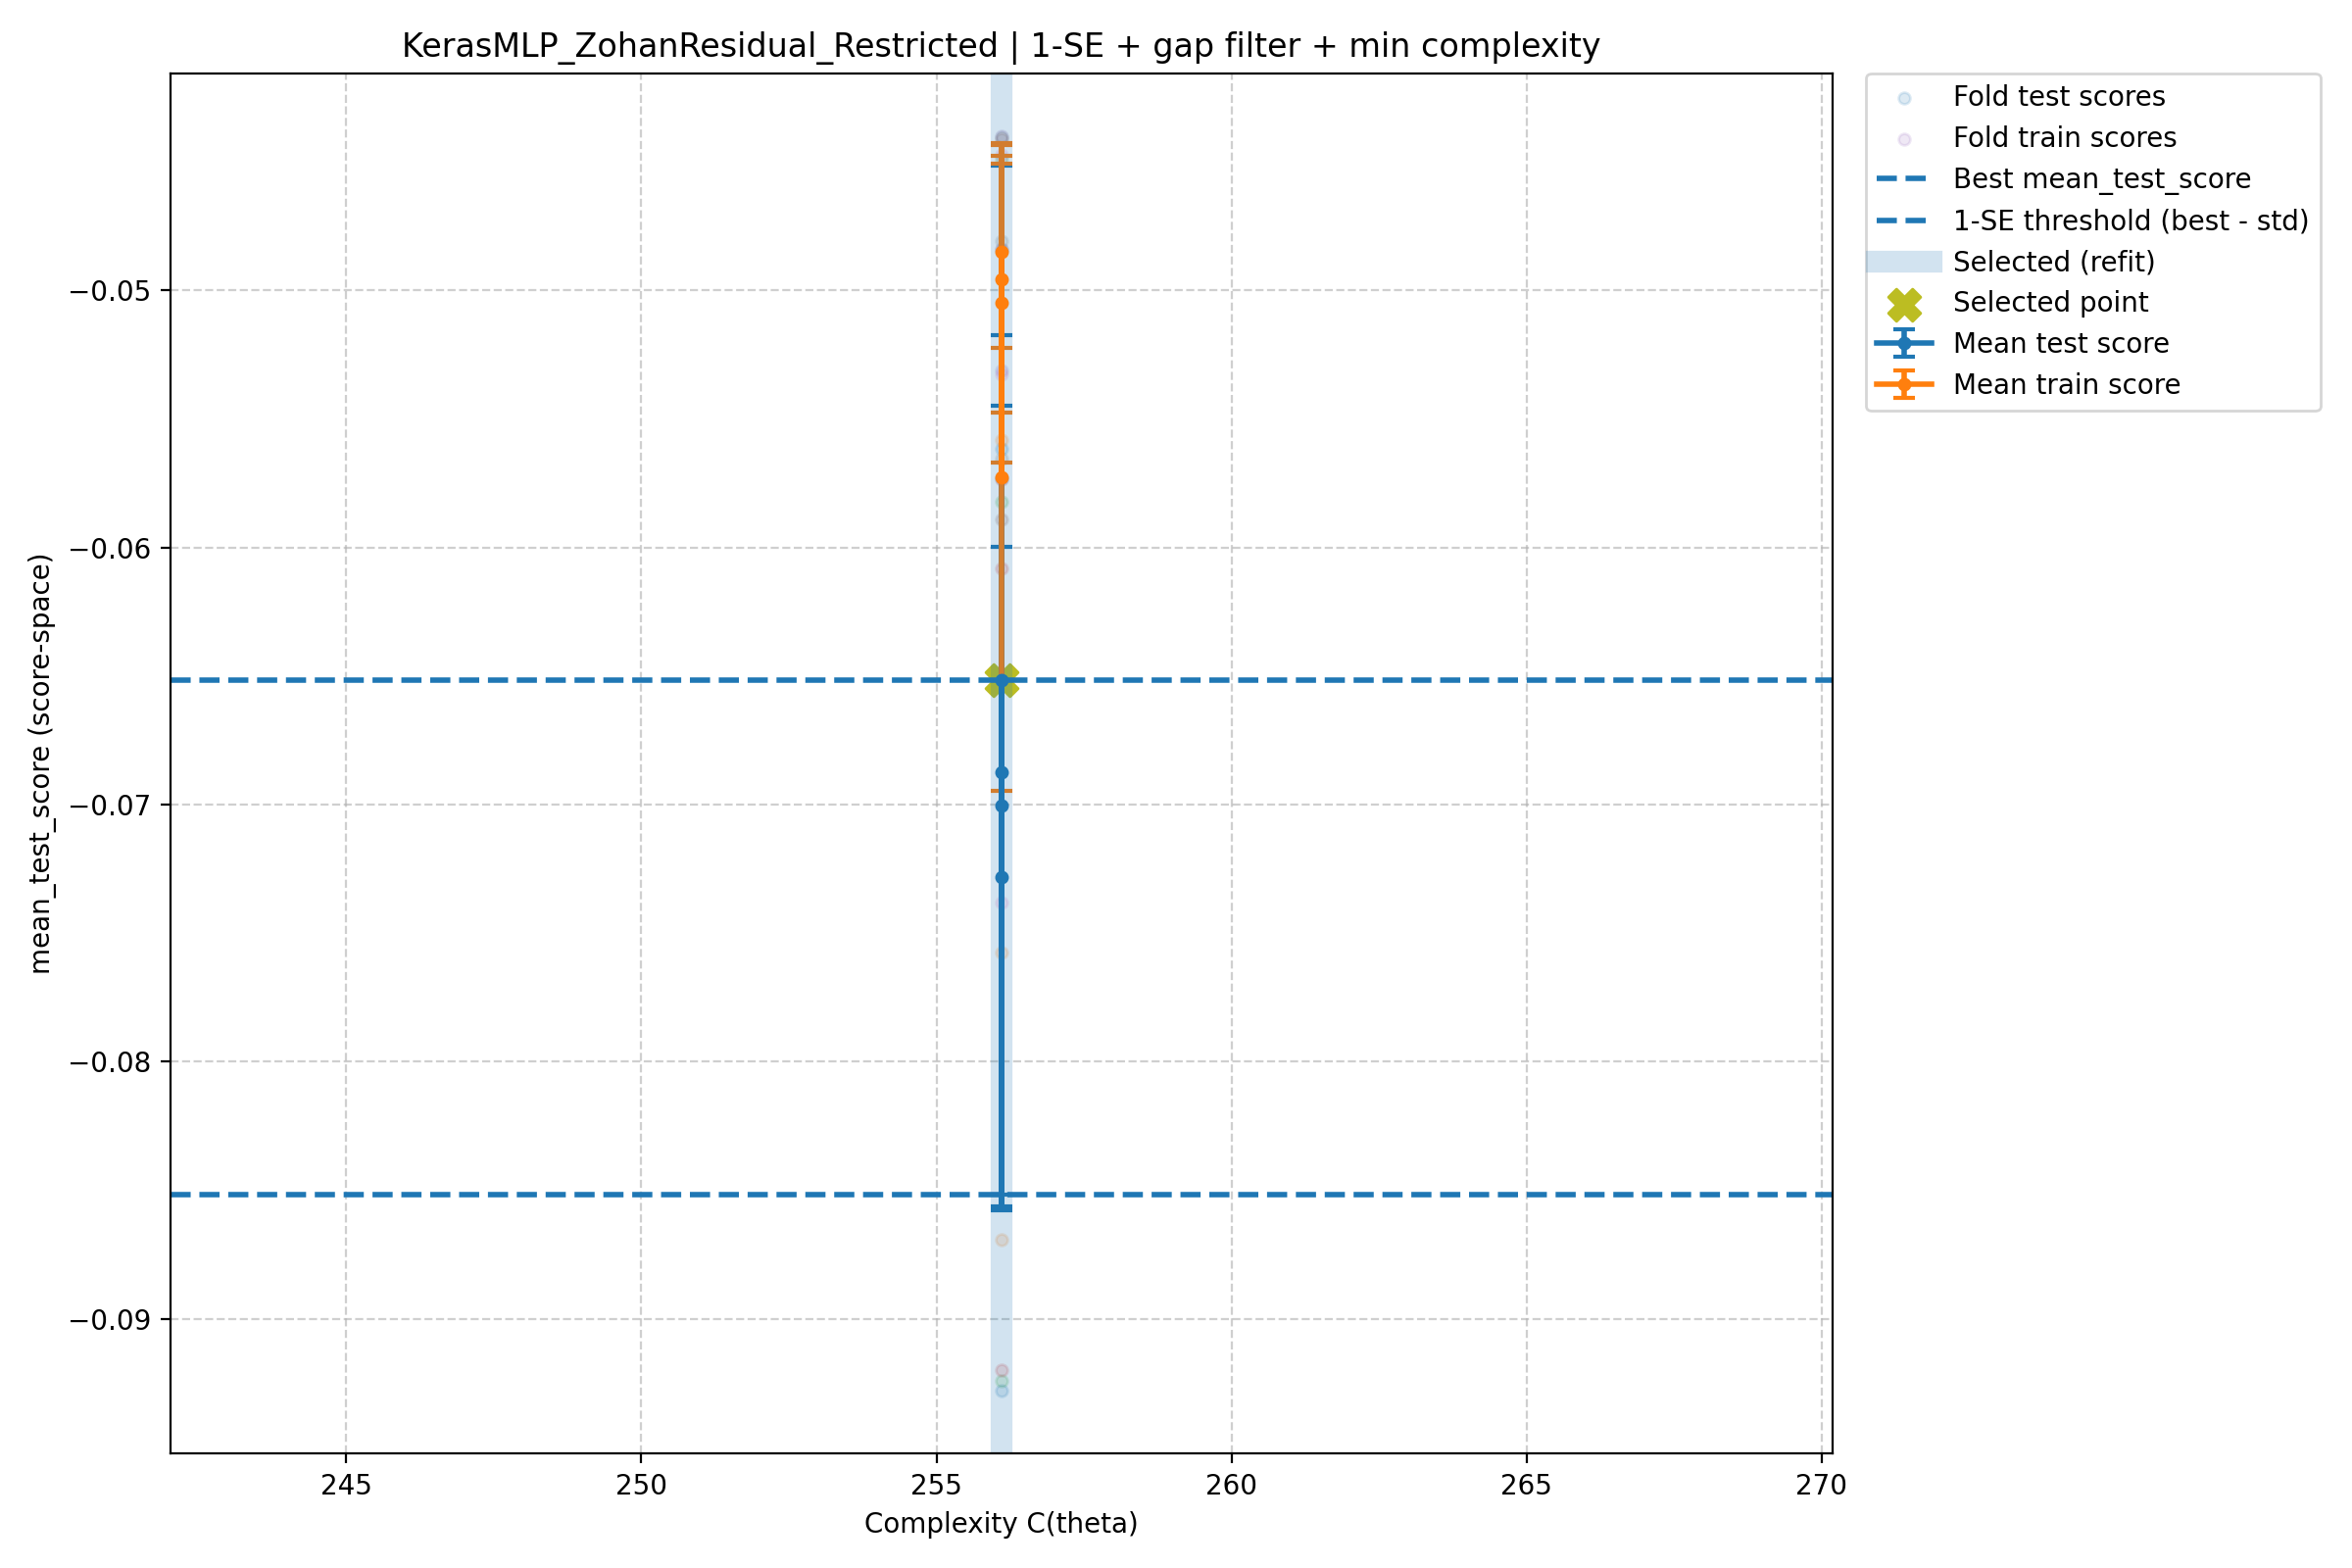
\includegraphics[width=0.85\textwidth]{tcc_images/chap06/model_selection/selection_PhyResidual.png}
\end{slide}
%========================================================================
\begin{slide}{Apêndice — Comparação Stage 2 (RMSE)}
  \centering
  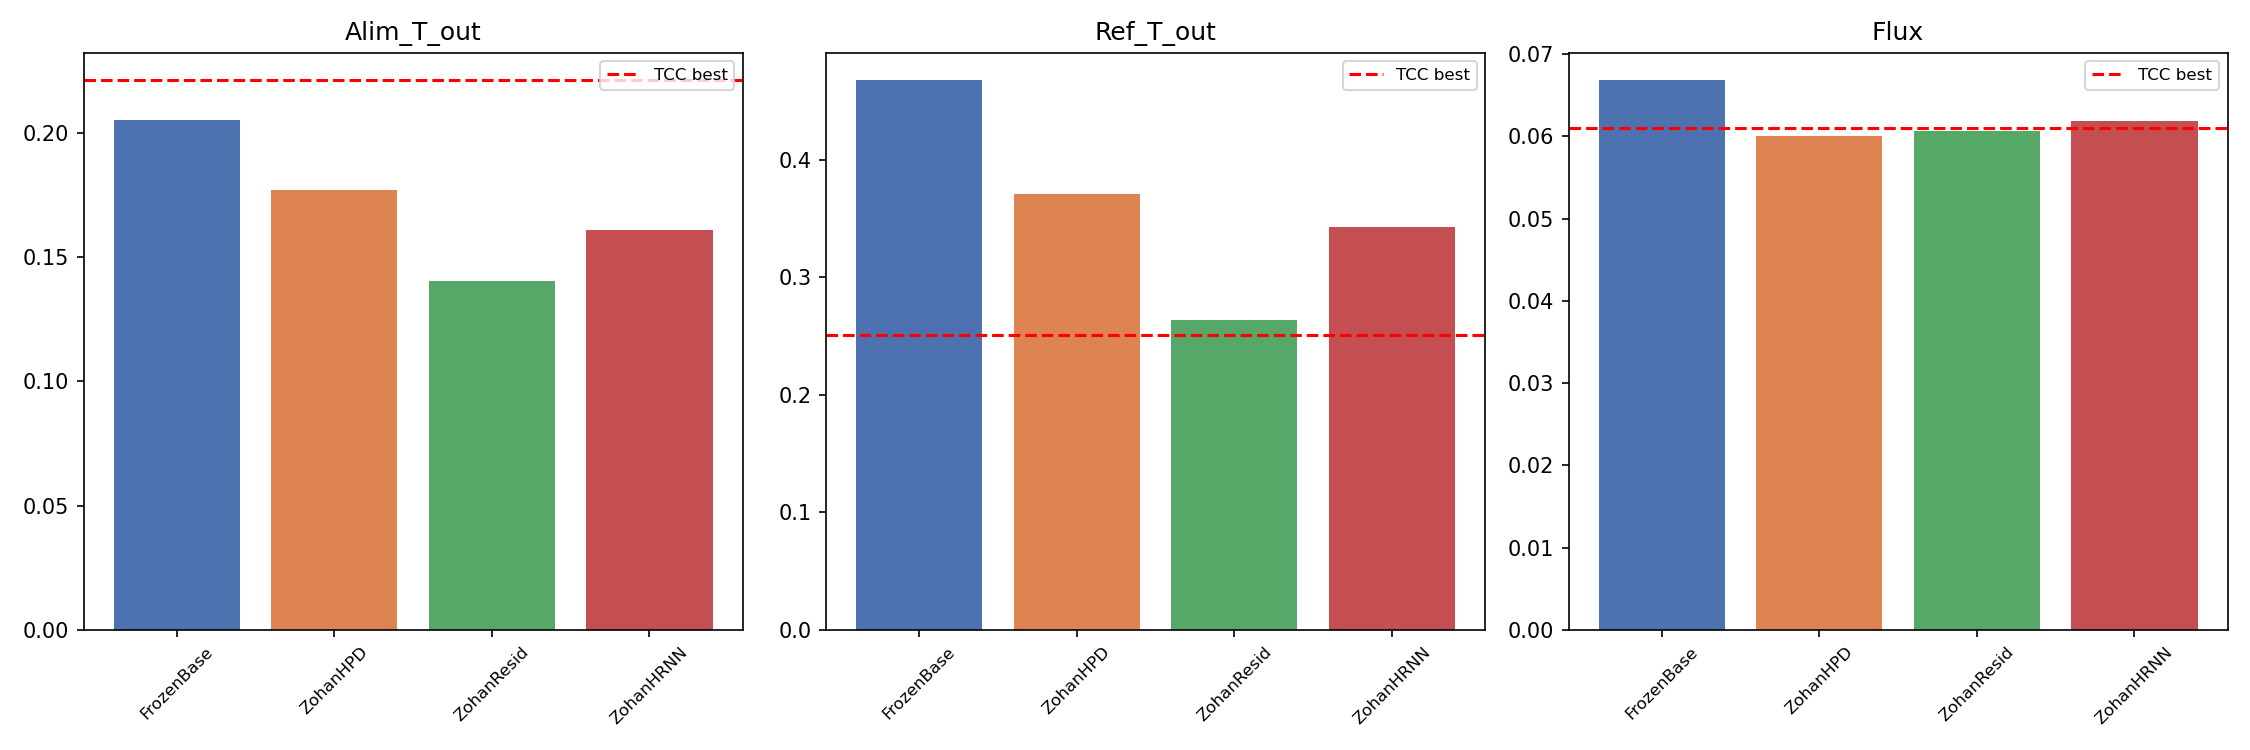
\includegraphics[width=0.85\textwidth]{tcc_images/chap06/model_selection/rmse_stage2_comparacao.png}
\end{slide}
%========================================================================
\begin{slide}{Apêndice — Stage 0: Modelos Lineares}
  \centering
  \scriptsize
  \begin{tabular}{llcccccc}
    \toprule
    \textbf{Modelo} & \textbf{Alvo} & \multicolumn{3}{c}{\textbf{CV RMSE}} & \multicolumn{3}{c}{\textbf{Test RMSE}} \\
    \cmidrule(lr){3-5} \cmidrule(lr){6-8}
    & & T$_{alim}$ & T$_{ref}$ & Flux & T$_{alim}$ & T$_{ref}$ & Flux \\
    \midrule
    OLS & --- & \textbf{0,196} & \textbf{0,240} & \textbf{0,081} & \cellcolor{blue!10}\textbf{0,231} & 0,227 & 0,077 \\
    \midrule
    Ridge & Alim & 0,225 & 0,448 & 0,094 & 0,274 & 0,407 & 0,075 \\
    \midrule
    Ridge & Ref & 0,195 & \cellcolor{yellow!15}0,244 & 0,082 & 0,232 & \cellcolor{orange!10}\textbf{0,219} & 0,076 \\
    \midrule
    Ridge & Flux & 0,225 & 0,448 & 0,094 & 0,274 & 0,407 & 0,075 \\
    \midrule
    Lasso & Alim & 0,197 & 0,275 & 0,084 & 0,233 & 0,240 & 0,077 \\
    \midrule
    Lasso & Ref & 0,200 & 0,270 & 0,084 & 0,236 & 0,235 & 0,077 \\
    \midrule
    Lasso & Flux & 0,200 & 0,275 & 0,082 & 0,236 & 0,240 & \cellcolor{green!10}\textbf{0,075} \\
    \midrule
    ElasticNet & Alim & 0,364 & 0,656 & 0,126 & 0,385 & 0,649 & 0,090 \\
    \midrule
    ElasticNet & Ref & 0,197 & 0,268 & 0,082 & 0,233 & 0,232 & 0,075 \\
    \midrule
    ElasticNet & Flux & 0,281 & 0,528 & 0,109 & 0,316 & 0,481 & 0,081 \\
    \bottomrule
  \end{tabular}
\end{slide}
%========================================================================
\begin{slide}{Apêndice — Stage 0: Árvores de Decisão}
  \centering
  \scriptsize
  \begin{tabular}{llcccccc}
    \toprule
    \textbf{Modelo} & \textbf{Alvo} & \multicolumn{3}{c}{\textbf{CV RMSE}} & \multicolumn{3}{c}{\textbf{Test RMSE}} \\
    \cmidrule(lr){3-5} \cmidrule(lr){6-8}
    & & T$_{alim}$ & T$_{ref}$ & Flux & T$_{alim}$ & T$_{ref}$ & Flux \\
    \midrule
    DT & Alim & 0,793 & 1,471 & 0,485 & 0,683 & 1,150 & 0,300 \\
    \midrule
    DT & Ref & 1,059 & 1,464 & 0,504 & 0,836 & 1,197 & 0,310 \\
    \midrule
    DT & Flux & 1,099 & 2,260 & 0,572 & 1,149 & 1,956 & 0,372 \\
    \midrule
    RF & Alim & 0,900 & 1,455 & 0,434 & 0,829 & 1,144 & 0,292 \\
    \midrule
    RF & Ref & 0,799 & 1,137 & 0,422 & 0,652 & 0,859 & 0,263 \\
    \midrule
    RF & Flux & 1,019 & 2,240 & 0,419 & 0,989 & 2,042 & 0,300 \\
    \midrule
    GB & Alim & \textbf{0,614} & 0,484 & 0,358 & \cellcolor{blue!10}\textbf{0,406} & \cellcolor{orange!10}\textbf{0,309} & 0,193 \\
    \midrule
    GB & Ref & 0,618 & 0,468 & 0,358 & 0,417 & 0,324 & 0,198 \\
    \midrule
    GB & Flux & 0,632 & \textbf{0,465} & \textbf{0,344} & 0,429 & 0,286 & \cellcolor{green!10}\textbf{0,190} \\
    \bottomrule
  \end{tabular}
\end{slide}
%========================================================================
\begin{slide}{Apêndice — Stage 1: Redes Neurais}
  \centering
  \scriptsize
  \begin{tabular}{llcccccc}
    \toprule
    \textbf{Arquitetura} & \textbf{Alvo} & \multicolumn{3}{c}{\textbf{CV RMSE}} & \multicolumn{3}{c}{\textbf{Test RMSE}} \\
    \cmidrule(lr){3-5} \cmidrule(lr){6-8}
    & & T$_{alim}$ & T$_{ref}$ & Flux & T$_{alim}$ & T$_{ref}$ & Flux \\
    \midrule
    (128,64), tanh, lr=0,001, l2=0,001 & Alim & 0,260 & \textbf{0,445} & 0,115 & 0,215 & \cellcolor{orange!10}\textbf{0,309} & 0,073 \\
    (128,64), tanh, lr=0,001, l2=0,001 & Ref & 0,267 & 0,459 & 0,116 & 0,227 & 0,318 & 0,073 \\
    (128,64,32), relu, lr=0,003, l2=0,0 & Flux & \textbf{0,222} & 0,554 & \textbf{0,081} & \cellcolor{blue!10}\textbf{0,178} & 0,369 & \cellcolor{green!10}\textbf{0,066} \\
    \bottomrule
  \end{tabular}
\end{slide}
%========================================================================
\begin{slide}{Apêndice — Stage 2: Modelos Híbridos}
  \centering
  \scriptsize
  \begin{tabular}{llcccccc}
    \toprule
    \textbf{Modelo} & \textbf{Alvo} & \multicolumn{3}{c}{\textbf{CV RMSE}} & \multicolumn{3}{c}{\textbf{Test RMSE}} \\
    \cmidrule(lr){3-5} \cmidrule(lr){6-8}
    & & T$_{alim}$ & T$_{ref}$ & Flux & T$_{alim}$ & T$_{ref}$ & Flux \\
    \midrule
    \textbf{PhyResidual} & \textbf{Alim} & 0,275 & \textbf{0,301} & \textbf{0,060} & 0,225 & 0,222 & 0,057 \\
    \textbf{PhyResidual} & \textbf{Ref} & 0,274 & 0,305 & 0,061 & 0,224 & 0,231 & 0,058 \\
    \rowcolor{green!6}
    \textbf{PhyResidual} & \textbf{Flux} & \textbf{0,236} & 0,346 & 0,072 & \cellcolor{blue!10}\textbf{0,183} & \cellcolor{orange!10}\textbf{0,214} & \cellcolor{green!10}\textbf{0,054} \\
    PhyHybrid & Alim & 0,273 & 0,306 & 0,061 & 0,224 & 0,231 & 0,058 \\
    PhyHybrid & Ref & 0,275 & 0,302 & 0,061 & 0,225 & 0,230 & 0,058 \\
    PhyHybrid & Flux & 0,284 & 0,399 & 0,075 & 0,222 & 0,239 & 0,055 \\
    PhyInput & Alim & 0,273 & 0,325 & 0,098 & 0,213 & 0,250 & 0,064 \\
    PhyInput & Ref & 0,275 & 0,432 & 0,106 & 0,216 & 0,269 & 0,066 \\
    PhyInput & Flux & 0,260 & 0,625 & 0,104 & 0,213 & 0,426 & 0,063 \\
    \midrule
    PhyLoss ($\omega{=}0{,}0$) & Alim & 0,180 & 0,348 & 0,067 & 0,188 & 0,350 & 0,068 \\
    PhyLoss ($\omega{=}0{,}7$) & Ref  & 0,310 & 0,250 & 0,192 & 0,340 & 0,286 & 0,220 \\
    PhyLoss ($\omega{=}0{,}0$) & Flux & 0,203 & 0,422 & 0,066 & 0,226 & 0,438 & 0,069 \\
    \bottomrule
  \end{tabular}
\end{slide}
%========================================================================
\begin{slide}{Apêndice — Curva de Aprendizado (Baseline Alim e PhyResidual)}
  \centering
  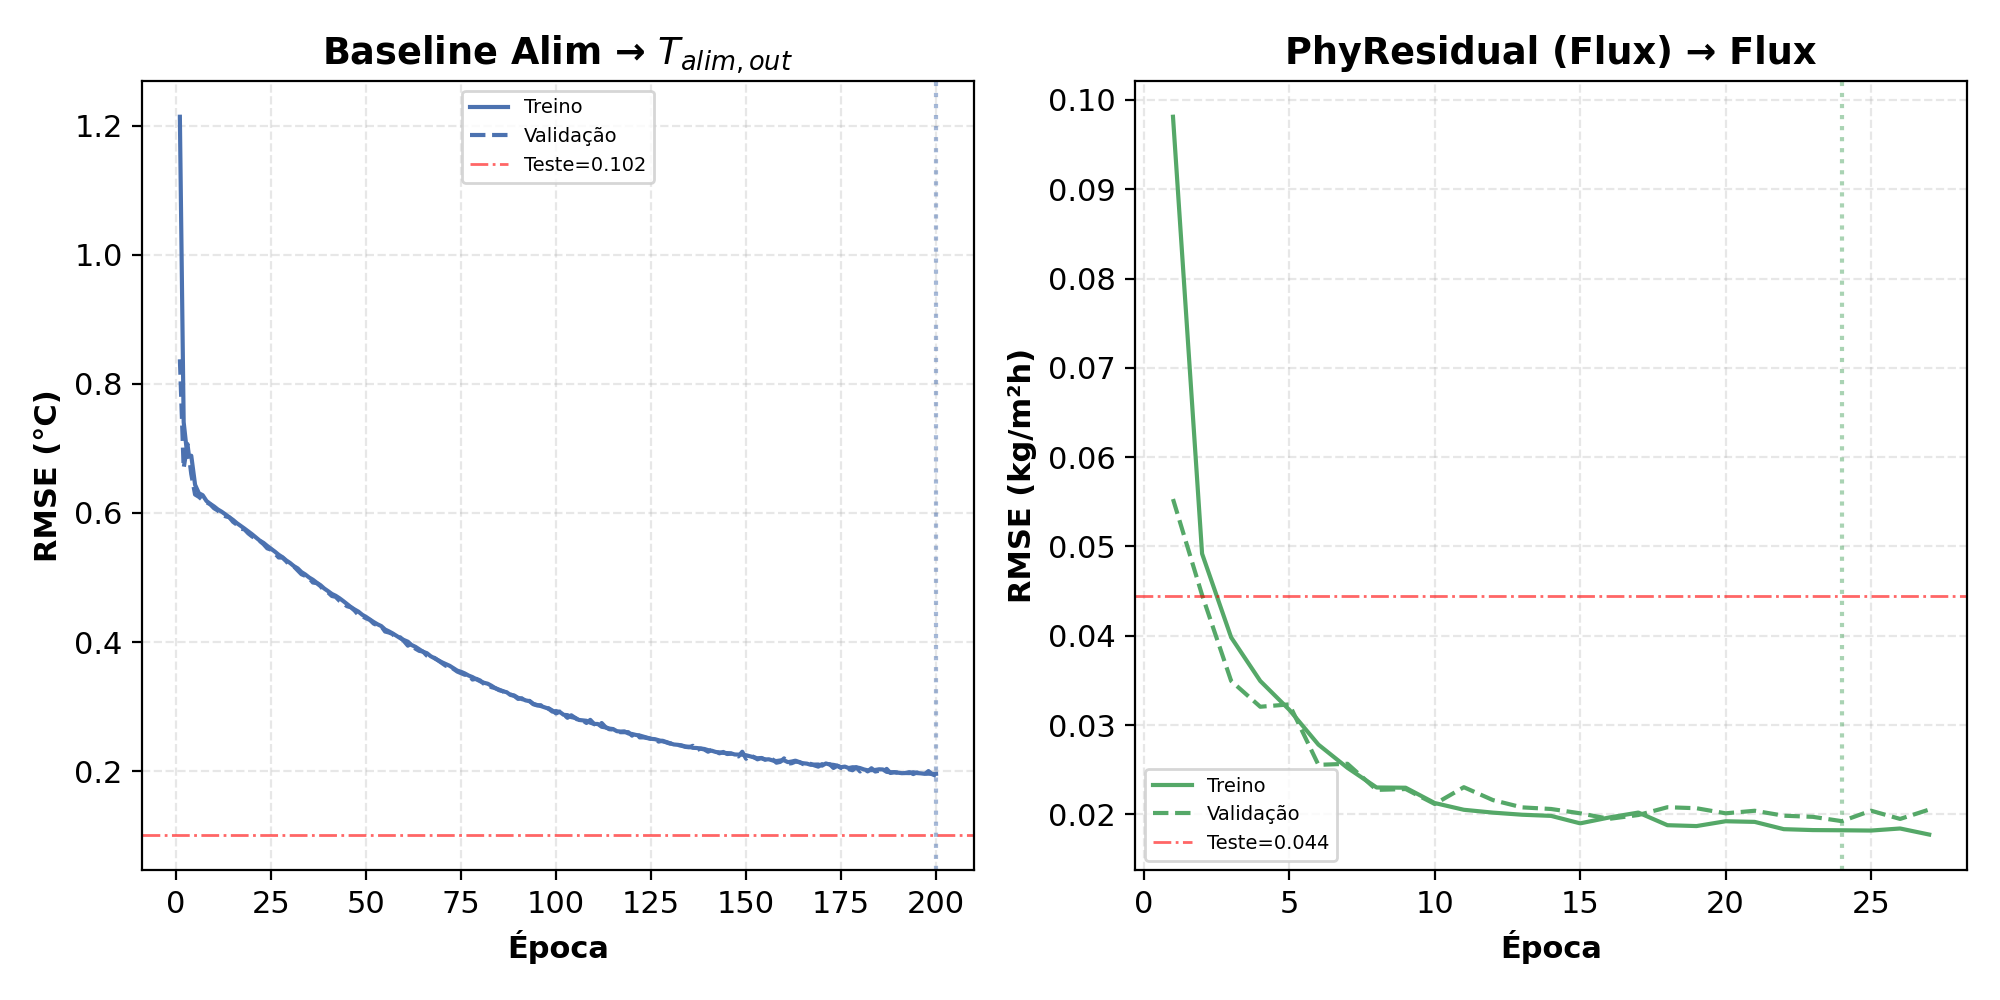
\includegraphics[width=0.85\textwidth]{tcc_images/chap06/model_selection/learning_curve_baseline_n_v3.png}
\end{slide}
